\documentclass[color=usenames,dvipsnames]{beamer}\usepackage[]{graphicx}\usepackage[]{color}
%% maxwidth is the original width if it is less than linewidth
%% otherwise use linewidth (to make sure the graphics do not exceed the margin)
\makeatletter
\def\maxwidth{ %
  \ifdim\Gin@nat@width>\linewidth
    \linewidth
  \else
    \Gin@nat@width
  \fi
}
\makeatother

\definecolor{fgcolor}{rgb}{0, 0, 0}
\newcommand{\hlnum}[1]{\textcolor[rgb]{0.69,0.494,0}{#1}}%
\newcommand{\hlstr}[1]{\textcolor[rgb]{0.749,0.012,0.012}{#1}}%
\newcommand{\hlcom}[1]{\textcolor[rgb]{0.514,0.506,0.514}{\textit{#1}}}%
\newcommand{\hlopt}[1]{\textcolor[rgb]{0,0,0}{#1}}%
\newcommand{\hlstd}[1]{\textcolor[rgb]{0,0,0}{#1}}%
\newcommand{\hlkwa}[1]{\textcolor[rgb]{0,0,0}{\textbf{#1}}}%
\newcommand{\hlkwb}[1]{\textcolor[rgb]{0,0.341,0.682}{#1}}%
\newcommand{\hlkwc}[1]{\textcolor[rgb]{0,0,0}{\textbf{#1}}}%
\newcommand{\hlkwd}[1]{\textcolor[rgb]{0.004,0.004,0.506}{#1}}%
\let\hlipl\hlkwb

\usepackage{framed}
\makeatletter
\newenvironment{kframe}{%
 \def\at@end@of@kframe{}%
 \ifinner\ifhmode%
  \def\at@end@of@kframe{\end{minipage}}%
  \begin{minipage}{\columnwidth}%
 \fi\fi%
 \def\FrameCommand##1{\hskip\@totalleftmargin \hskip-\fboxsep
 \colorbox{shadecolor}{##1}\hskip-\fboxsep
     % There is no \\@totalrightmargin, so:
     \hskip-\linewidth \hskip-\@totalleftmargin \hskip\columnwidth}%
 \MakeFramed {\advance\hsize-\width
   \@totalleftmargin\z@ \linewidth\hsize
   \@setminipage}}%
 {\par\unskip\endMakeFramed%
 \at@end@of@kframe}
\makeatother

\definecolor{shadecolor}{rgb}{.97, .97, .97}
\definecolor{messagecolor}{rgb}{0, 0, 0}
\definecolor{warningcolor}{rgb}{1, 0, 1}
\definecolor{errorcolor}{rgb}{1, 0, 0}
\newenvironment{knitrout}{}{} % an empty environment to be redefined in TeX

\usepackage{alltt}
%\documentclass[color=usenames,dvipsnames,handout]{beamer}


\usepackage[sans]{../../lab1}
\usepackage{bm}


\hypersetup{pdftex,pdfstartview=FitV}









%% New command for inline code that isn't to be evaluated
\definecolor{inlinecolor}{rgb}{0.878, 0.918, 0.933}
\newcommand{\inr}[1]{\colorbox{inlinecolor}{\texttt{#1}}}
\IfFileExists{upquote.sty}{\usepackage{upquote}}{}
\begin{document}


%\setlength\fboxsep{0pt}



\begin{frame}[plain]
  \huge
  \centering \par
  \textcolor{NavyBlue}{Introduction to Statistical Modeling} \\
  \vspace{1cm}
  \Large
  November 2 \& 5, 2018 \par
\end{frame}


\section{Motivation}


\begin{frame}
  \frametitle{Outline}
  \LARGE
   \only<1>{\tableofcontents[hideallsubsections]}
%   \only<2>{\tableofcontents[currentsection,hideallsubsections]}
\end{frame}



\begin{frame}
  \frametitle{Looking ahead}
  \Large
  \begin{itemize}
    \item Linear models
    \item[]
    \item Linear mixed effects models
    \item[]
    \item Generalized linear models
    \item[]
    \item Model selection and multi-model inference
    \item[]
    \item Goodness-of-fit
  \end{itemize}
\end{frame}




\begin{frame}
  \frametitle{Motivation}
  \large
  {\bf Why do we need this part of the course? \par}
  \pause
%\begin{enumerate}[<+- | visible@+->][\bf \color{PineGreen} (1)]
  \begin{itemize}[<+->]
    \item We have been modeling all along
    \item Good experimental design + ANOVA is usually the most direct
      route to causal inference
    \item Often, however, it isn't possible (or even desirable) to
      control some aspects of the system being investigated
    \item When manipulative experiments aren't %causal inference isn't
      possible, observational studies
      and predictive models are the next best option
  \end{itemize}
%\end{enumerate}
% Mention BLOGs
\end{frame}




%% \begin{frame}
%%   \frametitle{Assignment}
%% <<eval=true,echo=false,results=hide>>=
%% set.seed(894)
%% N <- 100
%% a <- 4
%% n <- N/a
%% x <- runif(N, 5, 20)
%% g <- gl(a, n, labels=c("Control", "Low", "Med", "High"))
%% #contrasts(g) <- c("contr.sum", "contr.poly")
%% dat <- data.frame(diet=g, length=x,
%%                   moon=sample(1:4, N, replace=TRUE),
%%                   sun=sample(1:10, N, replace=TRUE))
%% X <- model.matrix(~diet+length, dat)
%% X
%% beta <- c(20, 1, 2, 4, 0.5)
%% mu <- X %*% beta
%% mu
%% sigma <- 2
%% set.seed(52)
%% y <- rnorm(N, mu, sigma)
%% tapply(y, g, mean)
%% dat <- cbind(weight=y, dat)
%% #plot(weight ~ x, dat, col=rep(1:4, each=n))
%% #boxplot(weight ~ diet, dat)
%% write.csv(dat, "dietData.csv", row.names=FALSE)
%% @
%% \end{frame}




%\section{What is a model?}



\begin{frame}
  \frametitle{What is a model?}
%  \begin{block}
  \large
    {\bf Definition} \\
    A model is an abstraction of reality used to describe the
    relationship between two or more variables \par
%  \end{block}
    \pause
    \vfill %\vspace{0.5cm}
  {\bf Important point} \\
  ``All models are wrong but some are useful'' (George Box, 1976) \\
  \pause
  \vfill
  {\bf Types of models}
  \begin{itemize}
    \item Conceptual
    \item Mathematical
    \item Statistical
  \end{itemize}
\end{frame}




\begin{frame}
  \frametitle{Statistical models}
  \large
  {\bf What are they good for?}
  \begin{itemize}[<+->]
    \item Formalizing hypotheses using math and probability
    \item Evaulating hypotheses by confronting models with data
    \item Predicting future outcomes
  \end{itemize}
\end{frame}




\begin{frame}
  \frametitle{Statistical models}
  {\bf \large Two important pieces \par}
  \large
%  \begin{enumerate}[<+- | visible@+->][\bf \color{PineGreen} (1)]
  \begin{enumerate}[\bf \color{PineGreen} (1)]
    \large
    \item<1-> Deterministic component(s)
      \begin{itemize}
        \large
        \item Equation(s) for the expected value of the response
          variable, denoted $\mathbb{E}(y)$
%        \item Often a linear model (LM), but could be a generalized
%          linear model (GLM), a generalized additive (GAM), or a
%          genearlized linear mixed effects model (GLMM), etc\dots
      \end{itemize}
    \item[]
    \item<2-> Stochastic component(s)
      \begin{itemize}
        \large
        \item Probability distribution(s) describing the differences
          between the expected values and the observed values
        \item In parametric statistics, we assume we know the
          distribution, but not the parameters of the distribution
      \end{itemize}
  \end{enumerate}
\end{frame}




%% \begin{frame}
%%   \frametitle{Example}
%%   {\bf Motivation \\}
%%   Prey numbers appear to be declining in the core of the Florida panther's range \\
%%   \pause
%%   \vfill
%%   {\bf Questions \\}
%%   How do predation, changing hydrology and hunting regulations
%%   influence white-tailed deer population viability?
%% \end{frame}


%% \begin{frame}
%%   \frametitle{Example -- South Florida Deer Study}
%% %  \begin{center}
%% %  \vspace{-8mm}
%%   \begin{columns}
%%     \begin{column}{0.6\textwidth}
%% %      \large
%%         \normalsize
%%       {\bf Objectives}
%%       \begin{enumerate}
%%         \normalsize
%%         \item[{\bf (1)}] Understand how deer populations are influenced by:
%%         \begin{itemize}
%% %          \large
%%         \normalsize
%%           \item Predation
%%           \item Hydrology
%%           \item Hunting
%%         \end{itemize}
%%         \item[{\bf (2)}] Develop a camera-based monitoring program
%%       \end{enumerate}
%%     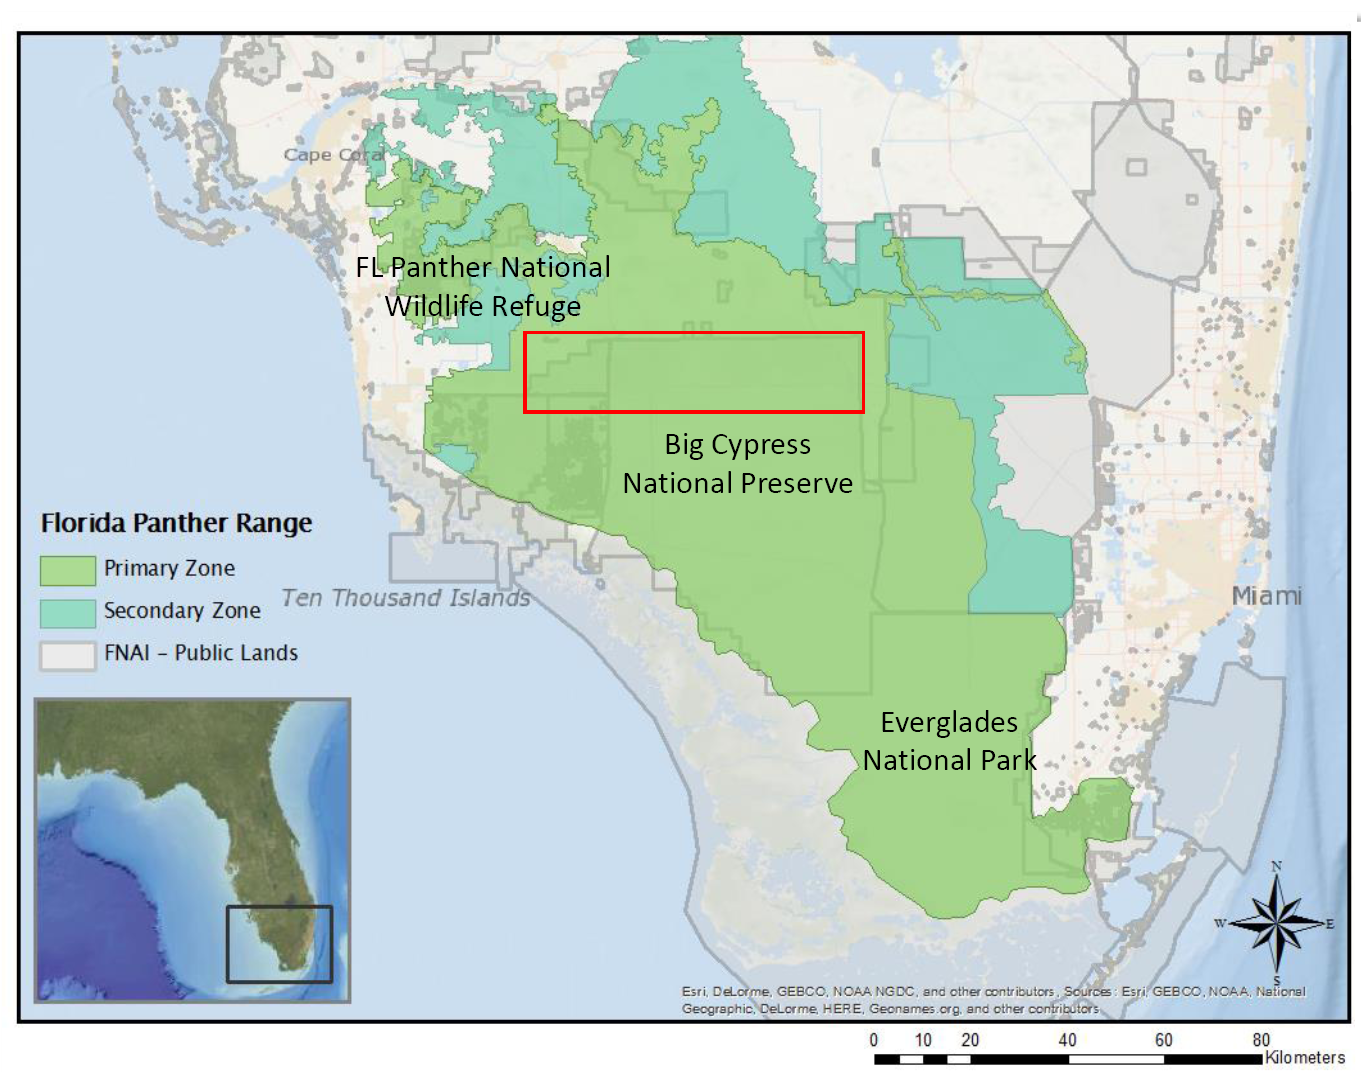
\includegraphics[width=0.9\textwidth]{figs/FL-study-area} \\ \vfill
%%     \end{column}
%%     \begin{column}{0.4\textwidth}
%%       \fbox{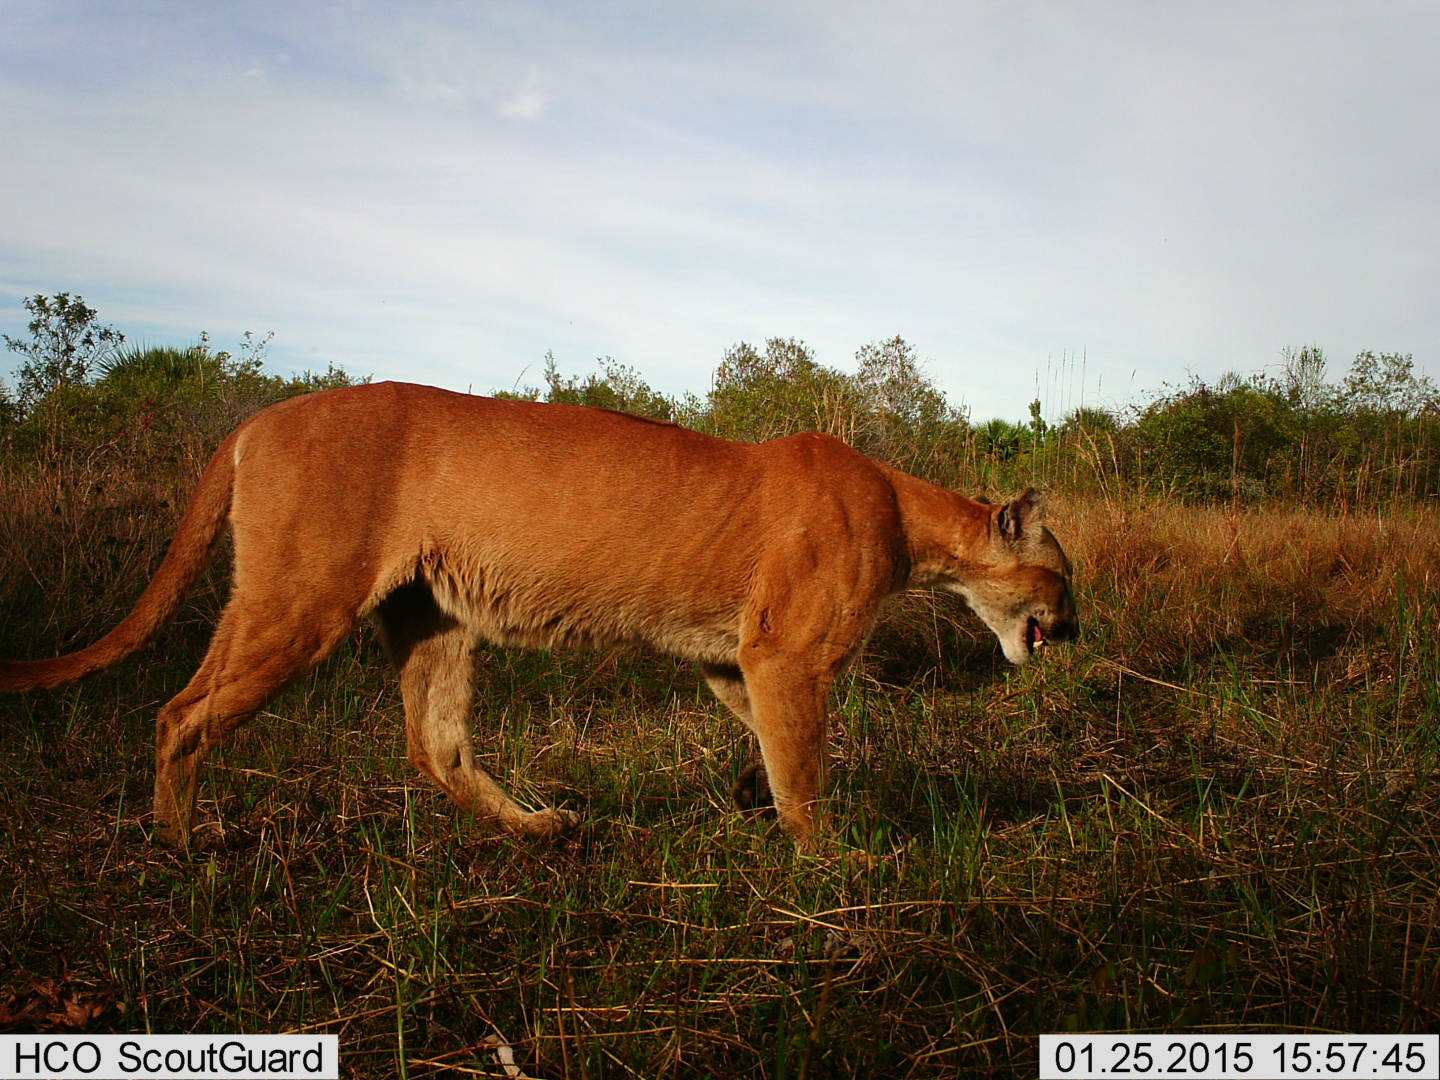
\includegraphics[width=\textwidth]{figs/puma1}} \\ \vfill
%%       \fbox{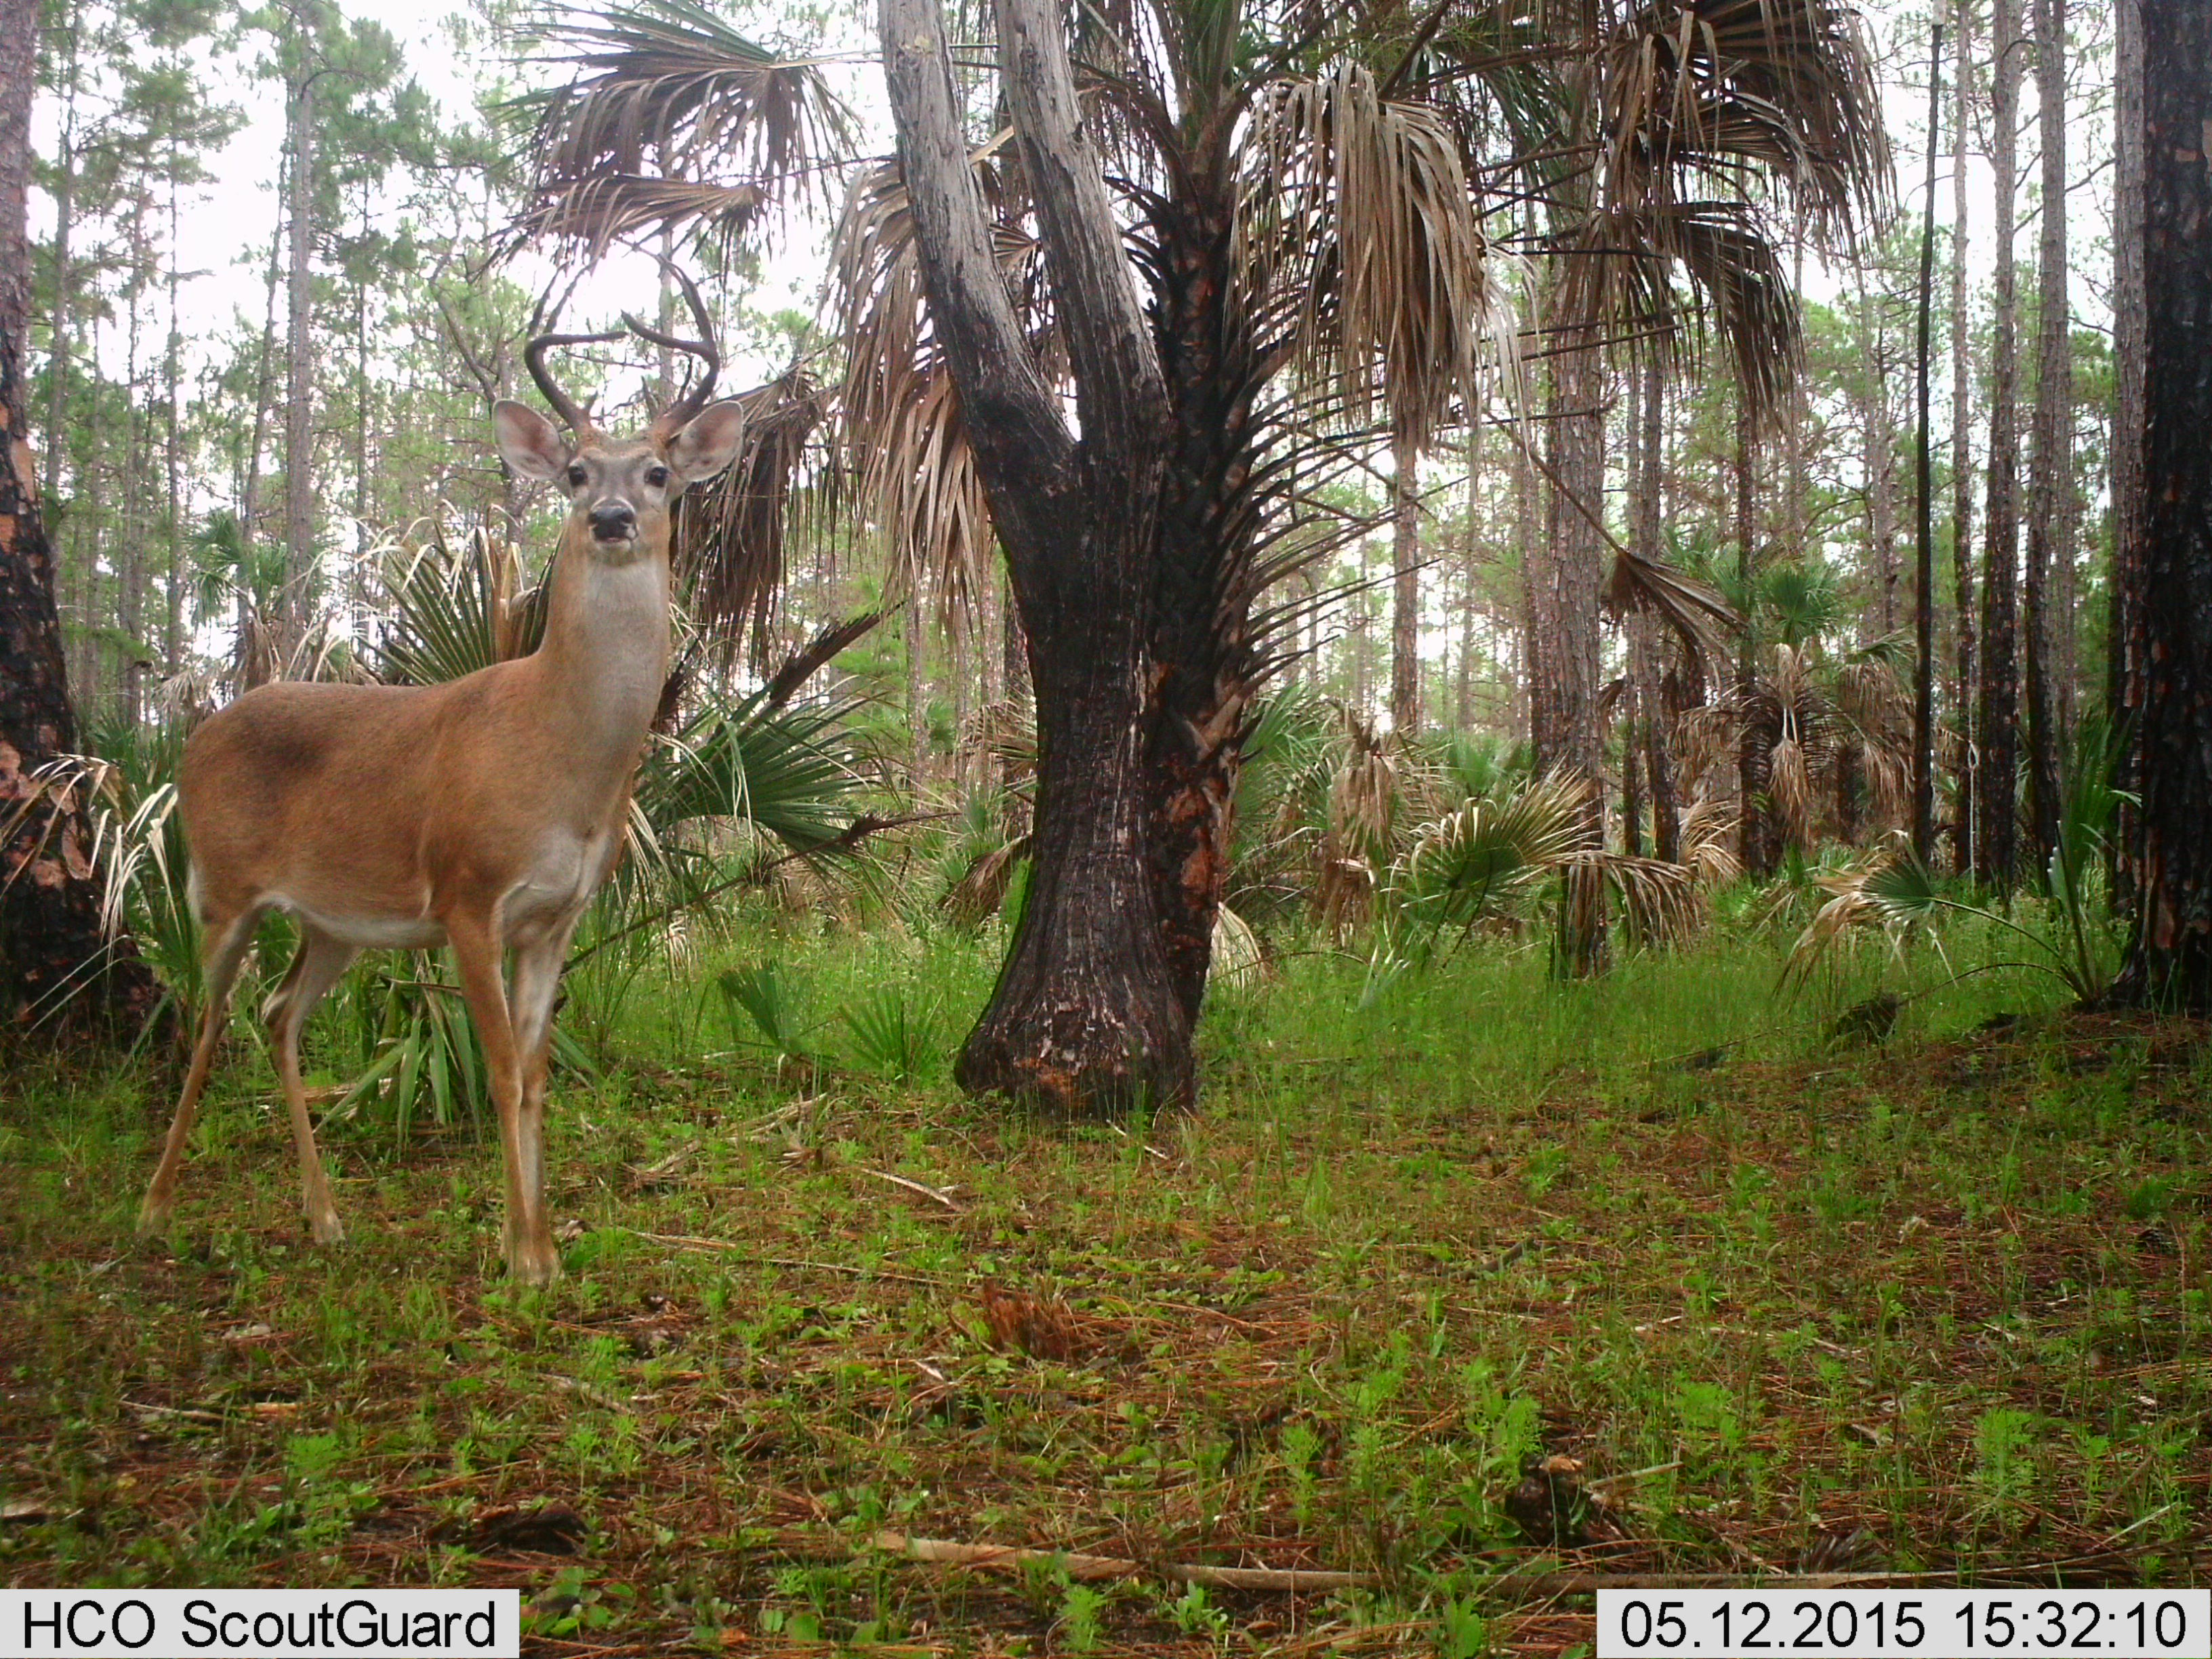
\includegraphics[width=\textwidth]{figs/2015-05-12-15-32-13_FP39}}
%%     \end{column}
%%   \end{columns}
%% %  \end{center}
%% \end{frame}









\section{Linear models}



\begin{frame}
  \frametitle{Outline}
  \LARGE
   \tableofcontents[currentsection,hideallsubsections]
\end{frame}



\begin{frame}[fragile]
  \frametitle{Is this a linear model?}
\[
y = 20 + 0.5 x
\]

\begin{center}
  \includegraphics[width=0.6\textwidth]{figure/linmod1-1}
\end{center}
\end{frame}




\begin{frame}[fragile]
  \frametitle{Is this a linear model?}
\[
y = 20 + 0.5 x - 0.3 x^2
\]

\begin{center}
  \includegraphics[width=0.6\textwidth]{figure/linmod2-1}
\end{center}
\end{frame}





\begin{frame}
  \frametitle{Linear model}
{\bf A linear model is an equation of the form:}

\[
y_i = \beta_0 + \beta_1 x_{i1} + \beta_2 x_{i2} + \ldots + \beta_p x_{ip} + \varepsilon_i
\]

where the $\beta$'s are coefficients, and the $x$ values are predictor
variables (or dummy variables for categorical predictors).
\pause

\vspace{0.5cm}

{\bf This equation is often expressed in matrix notation as:}

\[
{\bf y} = {\bf X} {\bm{\beta}} + {\bm \varepsilon}
\]

where $\bf X$ is a \alert{design matrix} and $\bm{\beta}$ is a
vector of coefficients.
\end{frame}


%\end{document}




\begin{frame}
  \frametitle{Linear model}
  {\bf All of the fixed effects models that we have covered can be
    expressed this way:}
  \[
  {\bf y} = {\bf X}{\bm \beta} + {\bm \varepsilon}
  \]
  {\bf where}
  \[
  {\bm \varepsilon} \sim \mbox{Normal}(0, \sigma^2)
  \]
  \pause
  \vfill
  {\bf Examples include} \\
  \begin{itemize}
    \item Completely randomized ANOVA
    \item Randomized complete block designs (when block effects are fixed)
    \item Factorial designs
    \item ANCOVA
  \end{itemize}
\end{frame}






\begin{frame}
  \frametitle{Then how do they differ?}
  \pause
  \large
  \begin{itemize}[<+->]
    \item The design matrices are different
    \item And so are the number of parameters (coefficients) to be
      estimated
    \item Important to understand how to construct design matrix that
      includes categorical variables
  \end{itemize}
\end{frame}




\begin{frame}%[fragile]
  \frametitle{Design matrix}
  \large
  \begin{itemize}[<+->]
    \item A design matrix usually has $N$ rows and $K$ colums, where $N$ is
      the total sample size and $K$ is the number of coefficients (parameters)
      to be estimated.
    \item The first column contains just 1's. This column corresponds
      to the intercept ($\beta_0$)
    \item Continuous predictor variables appear unchanged in the design matrix
    \item Categorical predictor variables appear as dummy variables
    \item In {\bf R}, the design matrix is created internally based on
      the formula that you provide
    \item The design matrix can be viewed using the {\tt model.matrix} function
  \end{itemize}
\end{frame}


\begin{frame}[fragile]
  \frametitle{Design matrix for linear regression}
  \begin{columns}
    \begin{column}{0.5\textwidth}
    {\bf Data}
      \scriptsize %\tiny
%<<>>=
%options(digits=2)
%@
\begin{knitrout}\scriptsize
\definecolor{shadecolor}{rgb}{0.878, 0.918, 0.933}\color{fgcolor}\begin{kframe}
\begin{alltt}
\hlstd{dietData} \hlkwb{<-} \hlkwd{read.csv}\hlstd{(}\hlstr{"dietData.csv"}\hlstd{)}
\hlkwd{head}\hlstd{(dietData,} \hlkwc{n}\hlstd{=}\hlnum{10}\hlstd{)}
\end{alltt}
\begin{verbatim}
##      weight    diet       age
## 1  23.83875 Control 11.622260
## 2  25.98799 Control 13.555397
## 3  30.29572 Control 15.357372
## 4  25.88463 Control  7.950214
## 5  18.48077 Control  5.493861
## 6  31.57542 Control 18.874970
## 7  23.79069 Control 12.811297
## 8  29.79574 Control 17.402436
## 9  21.66387 Control  7.379666
## 10 30.86618 Control 18.611817
\end{verbatim}
\end{kframe}
\end{knitrout}
    \end{column}
    \pause
    \begin{column}{0.5\textwidth}
      {\bf Design matrix}
      \scriptsize %\tiny
\begin{knitrout}\scriptsize
\definecolor{shadecolor}{rgb}{0.878, 0.918, 0.933}\color{fgcolor}\begin{kframe}
\begin{alltt}
\hlstd{X1} \hlkwb{<-} \hlkwd{model.matrix}\hlstd{(}\hlopt{~}\hlstd{age,}
                   \hlkwc{data}\hlstd{=dietData)}
\hlkwd{head}\hlstd{(X1,} \hlkwc{n}\hlstd{=}\hlnum{10}\hlstd{)}
\end{alltt}
\begin{verbatim}
##    (Intercept)       age
## 1            1 11.622260
## 2            1 13.555397
## 3            1 15.357372
## 4            1  7.950214
## 5            1  5.493861
## 6            1 18.874970
## 7            1 12.811297
## 8            1 17.402436
## 9            1  7.379666
## 10           1 18.611817
\end{verbatim}
\end{kframe}
\end{knitrout}
    \end{column}
  \end{columns}
  \pause
  \vfill
  {\centering \bf How do we multiply this design matrix ($\bf X$) by
    the vector of regression coefficients ($\bm \beta$)? \par}
\end{frame}






\begin{frame}
  \frametitle{Matrix multiplication}
  \Large
  \begin{center}
    \[
      \mathbb{E}(y) = {\bf X}{\bm \beta}
    \]
    \[
    \uncover<3->{
    \begin{bmatrix}
      aw + bx + cy + dz \\
      ew + fx + gy + hz \\
      iw + jx + ky + lz %\\
%      mw + nx + oy + pz
    \end{bmatrix}
    }
    \uncover<2->{=}
    \uncover<2->{
    \begin{bmatrix}
      a & b & c & d \\
      e & f & g & h \\
      i & j & k & l %\\
%      m & n & o & p
    \end{bmatrix}
    }
    \uncover<2->{
    \times
    \begin{bmatrix}
      w \\
      x \\
      y \\
      z
    \end{bmatrix}
    }
    \]
  \end{center}
  \normalsize
  \uncover<4->{
    {\bf In this example}}
    \begin{itemize}
      \item<4-> The first matrix corresponds to the expected values of $\bm y$
      \item<4-> The second matrix corresponds to the design matrix {$\bf X$}
      \item<4-> The third matrix (a column vector) corresponds to {$\bm \beta$}
    \end{itemize}
\end{frame}






\begin{frame}[fragile]
  \frametitle{Matrix multiplication}
{\bf \centering The vector of coefficients \par}
\small
\begin{knitrout}\small
\definecolor{shadecolor}{rgb}{0.878, 0.918, 0.933}\color{fgcolor}\begin{kframe}
\begin{alltt}
\hlstd{beta} \hlkwb{<-} \hlkwd{coef}\hlstd{(}\hlkwd{lm}\hlstd{(weight} \hlopt{~} \hlstd{age, dietData))}
\hlstd{beta}
\end{alltt}
\begin{verbatim}
## (Intercept)         age 
##   21.325234    0.518067
\end{verbatim}
\end{kframe}
\end{knitrout}
\pause
\large
\begin{center}
  {$\mathbb{E}({\bf y}) = {\bf X}{\bm \beta}$ or $y_i = \beta_0 + \beta_1 x_i$}
\end{center}
\pause
\small
\begin{knitrout}\small
\definecolor{shadecolor}{rgb}{0.878, 0.918, 0.933}\color{fgcolor}\begin{kframe}
\begin{alltt}
\hlstd{Ey1} \hlkwb{<-} \hlstd{X1} \hlopt \hlstd{beta}
\hlkwd{head}\hlstd{(Ey1,} \hlnum{5}\hlstd{)}
\end{alltt}
\begin{verbatim}
##       [,1]
## 1 27.34634
## 2 28.34784
## 3 29.28138
## 4 25.44398
## 5 24.17142
\end{verbatim}
\end{kframe}
\end{knitrout}
\end{frame}





%\subsection{Distributions}




%\subsection{Fixed effects models}



%% \begin{frame}
%%   \frametitle{Linear regression}
%% {\bf Deterministic part:}
%% %\[
%% %\mu_i = \mathbb{E}(\bf y) = \beta_0 + \beta_1x_i
%% %\]
%% %\pause
%% %{\bf The same thing, using matrix notation:}
%% \[
%% {\bm \mu} = \mathbb{E}(\bf y) = {\bf X}{\bm \beta}
%% \]
%% \pause
%% {\bf Stochastic part:}
%% %\[
%% %y_i \sim \mbox{Normal}(\mu_i, \sigma^2)
%% %\]
%% %\pause
%% %\centering or \par
%% \[
%% \varepsilon_i \sim \mbox{Normal}(0, \sigma^2)
%% \]
%% \end{frame}




%% \begin{frame}
%%   \frametitle{One-way ANOVA}
%% {\bf Deterministic part:}
%% \[
%% {\bm \mu} = \mathbb{E}(\bf y) = {\bf X}{\bm \beta}
%% \]
%% {\bf Stochastic part:}
%% %\[
%% %y_i \sim \mbox{Normal}(\mu_i, \sigma^2)
%% %\]
%% \[
%% \varepsilon_i \sim \mbox{Normal}(0, \sigma^2)
%% \]
%% \end{frame}




%% \begin{frame}
%%   \frametitle{A$\times$B Factorial ANOVA}
%% {\bf Deterministic part:}
%% \[
%% {\bm \mu} = \mathbb{E}(\bf y) = {\bf X}{\bm \beta}
%% \]
%% {\bf Stochastic part:}
%% %\[
%% %y_i \sim \mbox{Normal}(\mu_i, \sigma^2)
%% %\]
%% \[
%% \varepsilon_i \sim \mbox{Normal}(0, \sigma^2)
%% \]
%% \end{frame}



%% \begin{frame}
%%   \frametitle{A$\times$B$\times$C Factorial ANOVA}
%% {\bf Deterministic part:}
%% \[
%% {\bm \mu} = \mathbb{E}(\bf y) = {\bf X}{\bm \beta}
%% \]
%% {\bf Stochastic part:}
%% %\[
%% %y_i \sim \mbox{Normal}(\mu_i, \sigma^2)
%% %\]
%% \[
%% \varepsilon_i \sim \mbox{Normal}(0, \sigma^2)
%% \]
%% \end{frame}



%% \begin{frame}
%%   \frametitle{ANCOVA}
%% {\bf Deterministic part:}
%% \[
%% {\bm \mu} = \mathbb{E}(\bf y) = {\bf X}{\bm \beta}
%% \]
%% {\bf Stochastic part:}
%% %\[
%% %y_i \sim \mbox{Normal}(\mu_i, \sigma^2)
%% %\]
%% \[
%% \varepsilon_i \sim \mbox{Normal}(0, \sigma^2)
%% \]
%% \end{frame}



%% \begin{frame}
%%   \frametitle{Another equivalent expression}
%%   {\bf General linear model}
%%   \[
%%   {\bf y} = {\bf X}{\bm \beta} + {\bm \epsilon}
%%   \]
%%   {\bf where}
%%   \[
%%   {\bm \epsilon} \sim \mbox{Normal}(0, {\bf I}\sigma^2)
%%   \]
%% \end{frame}




\begin{frame}[fragile]
  \frametitle{One-way ANOVA}
  \scriptsize %\tiny
\begin{knitrout}\scriptsize
\definecolor{shadecolor}{rgb}{0.878, 0.918, 0.933}\color{fgcolor}\begin{kframe}
\begin{alltt}
\hlstd{lm2} \hlkwb{<-} \hlkwd{lm}\hlstd{(weight} \hlopt{~} \hlstd{diet,} \hlkwc{data}\hlstd{=dietData)}
\hlkwd{summary}\hlstd{(lm2)}
\end{alltt}
\begin{verbatim}
## 
## Call:
## lm(formula = weight ~ diet, data = dietData)
## 
## Residuals:
##     Min      1Q  Median      3Q     Max 
## -7.6371 -1.9253 -0.0366  1.9770  5.4576 
## 
## Coefficients:
##             Estimate Std. Error t value Pr(>|t|)    
## (Intercept)  26.1178     0.7691  33.958   <2e-16 ***
## dietHigh      2.5292     1.0877   2.325   0.0237 *  
## dietLow       0.4559     1.0877   0.419   0.6767    
## dietMed       1.1021     1.0877   1.013   0.3153    
## ---
## Signif. codes:  0 '***' 0.001 '**' 0.01 '*' 0.05 '.' 0.1 ' ' 1
## 
## Residual standard error: 2.979 on 56 degrees of freedom
## Multiple R-squared:  0.09908,	Adjusted R-squared:  0.05082 
## F-statistic: 2.053 on 3 and 56 DF,  p-value: 0.1169
\end{verbatim}
\end{kframe}
\end{knitrout}
\end{frame}



\begin{frame}[fragile]
  \frametitle{One-way ANOVA: Design matrix}
\begin{knitrout}
\definecolor{shadecolor}{rgb}{0.878, 0.918, 0.933}\color{fgcolor}\begin{kframe}
\begin{alltt}
\hlstd{X2} \hlkwb{<-} \hlkwd{model.matrix}\hlstd{(}\hlopt{~}\hlstd{diet,} \hlkwc{data}\hlstd{=dietData)}
\hlstd{X2[}\hlnum{20}\hlopt{:}\hlnum{30}\hlstd{,]}
\end{alltt}
\begin{verbatim}
##    (Intercept) dietHigh dietLow dietMed
## 20           1        0       1       0
## 21           1        0       1       0
## 22           1        0       1       0
## 23           1        0       1       0
## 24           1        0       1       0
## 25           1        0       1       0
## 26           1        0       1       0
## 27           1        0       1       0
## 28           1        0       1       0
## 29           1        0       1       0
## 30           1        0       1       0
\end{verbatim}
\end{kframe}
\end{knitrout}
\end{frame}


\begin{frame}[fragile]
  \frametitle{One-way ANOVA: Expected values of $y$}
  \footnotesize %\scriptsize
\begin{knitrout}\footnotesize
\definecolor{shadecolor}{rgb}{0.878, 0.918, 0.933}\color{fgcolor}\begin{kframe}
\begin{alltt}
\hlstd{betas2} \hlkwb{<-} \hlkwd{coef}\hlstd{(lm2)}
\hlstd{betas2}
\end{alltt}
\begin{verbatim}
## (Intercept)    dietHigh     dietLow     dietMed 
##  26.1178280   2.5292436   0.4558565   1.1020553
\end{verbatim}
\end{kframe}
\end{knitrout}
\pause
\begin{knitrout}\footnotesize
\definecolor{shadecolor}{rgb}{0.878, 0.918, 0.933}\color{fgcolor}\begin{kframe}
\begin{alltt}
\hlstd{Ey2} \hlkwb{<-} \hlstd{X2} \hlopt \hlstd{betas2}
\hlkwd{head}\hlstd{(Ey2)}
\end{alltt}
\begin{verbatim}
##       [,1]
## 1 26.11783
## 2 26.11783
## 3 26.11783
## 4 26.11783
## 5 26.11783
## 6 26.11783
\end{verbatim}
\end{kframe}
\end{knitrout}
\end{frame}



\begin{frame}[fragile]
  \frametitle{ANCOVA}
  \vspace{-2mm}
  \scriptsize %\tiny
\begin{knitrout}\scriptsize
\definecolor{shadecolor}{rgb}{0.878, 0.918, 0.933}\color{fgcolor}\begin{kframe}
\begin{alltt}
\hlstd{lm3} \hlkwb{<-} \hlkwd{lm}\hlstd{(weight} \hlopt{~} \hlstd{age} \hlopt{+} \hlstd{diet,} \hlkwc{data}\hlstd{=dietData)}
\hlkwd{summary}\hlstd{(lm3)}
\end{alltt}
\begin{verbatim}
## 
## Call:
## lm(formula = weight ~ age + diet, data = dietData)
## 
## Residuals:
##     Min      1Q  Median      3Q     Max 
## -3.8214 -1.2213 -0.2519  1.2161  4.9185 
## 
## Coefficients:
##             Estimate Std. Error t value Pr(>|t|)    
## (Intercept)  19.1402     0.8858  21.607  < 2e-16 ***
## age           0.5573     0.0594   9.382 5.20e-13 ***
## dietHigh      3.0830     0.6832   4.513 3.41e-05 ***
## dietLow       1.3688     0.6875   1.991 0.051472 .  
## dietMed       2.5265     0.6973   3.623 0.000636 ***
## ---
## Signif. codes:  0 '***' 0.001 '**' 0.01 '*' 0.05 '.' 0.1 ' ' 1
## 
## Residual standard error: 1.864 on 55 degrees of freedom
## Multiple R-squared:  0.6536,	Adjusted R-squared:  0.6284 
## F-statistic: 25.94 on 4 and 55 DF,  p-value: 4.147e-12
\end{verbatim}
\end{kframe}
\end{knitrout}
\end{frame}



\begin{frame}[fragile]
  \frametitle{ANCOVA: Design matrix}
\begin{knitrout}
\definecolor{shadecolor}{rgb}{0.878, 0.918, 0.933}\color{fgcolor}\begin{kframe}
\begin{alltt}
\hlstd{X3} \hlkwb{<-} \hlkwd{model.matrix}\hlstd{(}\hlopt{~}\hlstd{age}\hlopt{+}\hlstd{diet,} \hlkwc{data}\hlstd{=dietData)}
\hlstd{X3[}\hlnum{20}\hlopt{:}\hlnum{30}\hlstd{,]}
\end{alltt}
\begin{verbatim}
##    (Intercept)       age dietHigh dietLow dietMed
## 20           1  8.624227        0       1       0
## 21           1 10.259516        0       1       0
## 22           1 10.536797        0       1       0
## 23           1 15.114452        0       1       0
## 24           1 15.057981        0       1       0
## 25           1  9.515444        0       1       0
## 26           1  8.968441        0       1       0
## 27           1  5.010545        0       1       0
## 28           1  5.714703        0       1       0
## 29           1 11.964920        0       1       0
## 30           1 14.035229        0       1       0
\end{verbatim}
\end{kframe}
\end{knitrout}
\end{frame}




\begin{frame}[fragile]
  \frametitle{ANCOVA: Expected values of $y$}
  \footnotesize
\begin{knitrout}\footnotesize
\definecolor{shadecolor}{rgb}{0.878, 0.918, 0.933}\color{fgcolor}\begin{kframe}
\begin{alltt}
\hlstd{betas3} \hlkwb{<-} \hlkwd{coef}\hlstd{(lm3)}
\hlstd{betas3}
\end{alltt}
\begin{verbatim}
## (Intercept)         age    dietHigh     dietLow     dietMed 
##  19.1401563   0.5573171   3.0830412   1.3687607   2.5264570
\end{verbatim}
\end{kframe}
\end{knitrout}
\begin{knitrout}\footnotesize
\definecolor{shadecolor}{rgb}{0.878, 0.918, 0.933}\color{fgcolor}\begin{kframe}
\begin{alltt}
\hlstd{Ey3} \hlkwb{<-} \hlstd{X3} \hlopt \hlstd{betas3}
\hlkwd{head}\hlstd{(Ey3)}
\end{alltt}
\begin{verbatim}
##       [,1]
## 1 25.61744
## 2 26.69481
## 3 27.69908
## 4 23.57095
## 5 22.20198
## 6 29.65950
\end{verbatim}
\end{kframe}
\end{knitrout}
\end{frame}



\begin{frame}[fragile]
  \frametitle{Beyond ANCOVA}
  {\bf Now the slopes differ for each treatment}
  \tiny
\begin{knitrout}\tiny
\definecolor{shadecolor}{rgb}{0.878, 0.918, 0.933}\color{fgcolor}\begin{kframe}
\begin{alltt}
\hlstd{lm4} \hlkwb{<-} \hlkwd{lm}\hlstd{(weight} \hlopt{~} \hlstd{diet} \hlopt{*} \hlstd{age,} \hlkwc{data}\hlstd{=dietData)}
\hlkwd{summary}\hlstd{(lm4)}
\end{alltt}
\begin{verbatim}
## 
## Call:
## lm(formula = weight ~ diet * age, data = dietData)
## 
## Residuals:
##     Min      1Q  Median      3Q     Max 
## -3.7370 -1.2585  0.1167  1.1039  4.9604 
## 
## Coefficients:
##              Estimate Std. Error t value Pr(>|t|)    
## (Intercept)  17.90749    1.39518  12.835  < 2e-16 ***
## dietHigh      4.12823    1.95637   2.110  0.03968 *  
## dietLow       2.82133    2.12190   1.330  0.18944    
## dietMed       5.37507    1.97816   2.717  0.00892 ** 
## age           0.65577    0.10452   6.274 7.09e-08 ***
## dietHigh:age -0.08219    0.15271  -0.538  0.59273    
## dietLow:age  -0.11866    0.17474  -0.679  0.50009    
## dietMed:age  -0.26063    0.16845  -1.547  0.12788    
## ---
## Signif. codes:  0 '***' 0.001 '**' 0.01 '*' 0.05 '.' 0.1 ' ' 1
## 
## Residual standard error: 1.874 on 52 degrees of freedom
## Multiple R-squared:  0.6691,	Adjusted R-squared:  0.6245 
## F-statistic: 15.02 on 7 and 52 DF,  p-value: 1.524e-10
\end{verbatim}
\end{kframe}
\end{knitrout}
\end{frame}




\begin{frame}[fragile]
  \frametitle{The associated design matrix}
  \tiny
\begin{knitrout}\tiny
\definecolor{shadecolor}{rgb}{0.878, 0.918, 0.933}\color{fgcolor}\begin{kframe}
\begin{alltt}
\hlstd{X4} \hlkwb{<-} \hlkwd{model.matrix}\hlstd{(}\hlopt{~} \hlstd{diet} \hlopt{*} \hlstd{age,} \hlkwc{data}\hlstd{=dietData)}
\hlstd{X4[}\hlnum{20}\hlopt{:}\hlnum{30}\hlstd{,]}
\end{alltt}
\begin{verbatim}
##    (Intercept) dietHigh dietLow dietMed       age dietHigh:age dietLow:age
## 20           1        0       1       0  8.624227            0    8.624227
## 21           1        0       1       0 10.259516            0   10.259516
## 22           1        0       1       0 10.536797            0   10.536797
## 23           1        0       1       0 15.114452            0   15.114452
## 24           1        0       1       0 15.057981            0   15.057981
## 25           1        0       1       0  9.515444            0    9.515444
## 26           1        0       1       0  8.968441            0    8.968441
## 27           1        0       1       0  5.010545            0    5.010545
## 28           1        0       1       0  5.714703            0    5.714703
## 29           1        0       1       0 11.964920            0   11.964920
## 30           1        0       1       0 14.035229            0   14.035229
##    dietMed:age
## 20           0
## 21           0
## 22           0
## 23           0
## 24           0
## 25           0
## 26           0
## 27           0
## 28           0
## 29           0
## 30           0
\end{verbatim}
\end{kframe}
\end{knitrout}
\pause
\begin{knitrout}
\definecolor{shadecolor}{rgb}{0.878, 0.918, 0.933}\color{fgcolor}\begin{kframe}
\begin{alltt}
\hlstd{betas4} \hlkwb{<-} \hlkwd{coef}\hlstd{(lm4)}
\hlstd{Ey4} \hlkwb{<-} \hlstd{X4} \hlopt \hlstd{betas4}
\end{alltt}
\end{kframe}
\end{knitrout}
\end{frame}





%% \begin{frame}[fragile]
%%   \frametitle{Beyond ANCOVA}
%%   {\bf ... and we test for a moon effect}
%%   \tiny
%% <<>>=
%% lm3 <- lm(weight ~ diet * age + moon, data=dietData)
%% summary(lm3)
%% @
%% \end{frame}


%% \begin{frame}
%%   \frametitle{Mixed effects models}
%% {\bf The notation is only slightly more complex}
%% \end{frame}



%\subsection{Mixed effects models}




\section{Example}



\begin{frame}[plain]
  \frametitle{Example}
  \Huge
  \begin{center}
    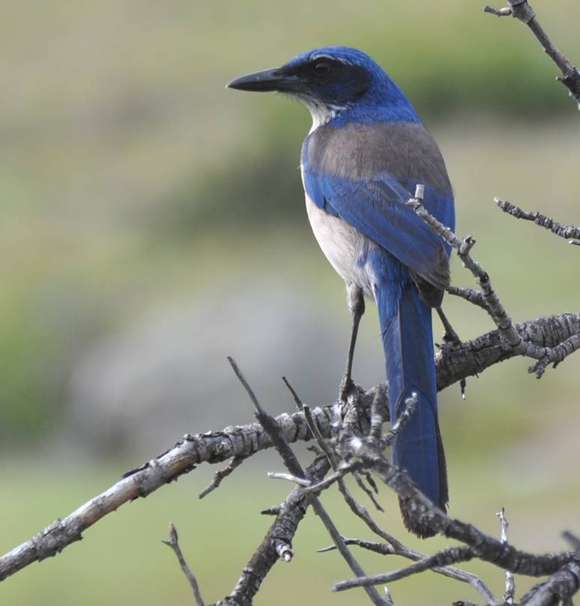
\includegraphics[width=0.5\textwidth]{figs/issj}
    The Island Scrub-Jay
  \end{center}
\end{frame}



\begin{frame}[plain]
  \frametitle{Example}
  \Huge
  \begin{center}
    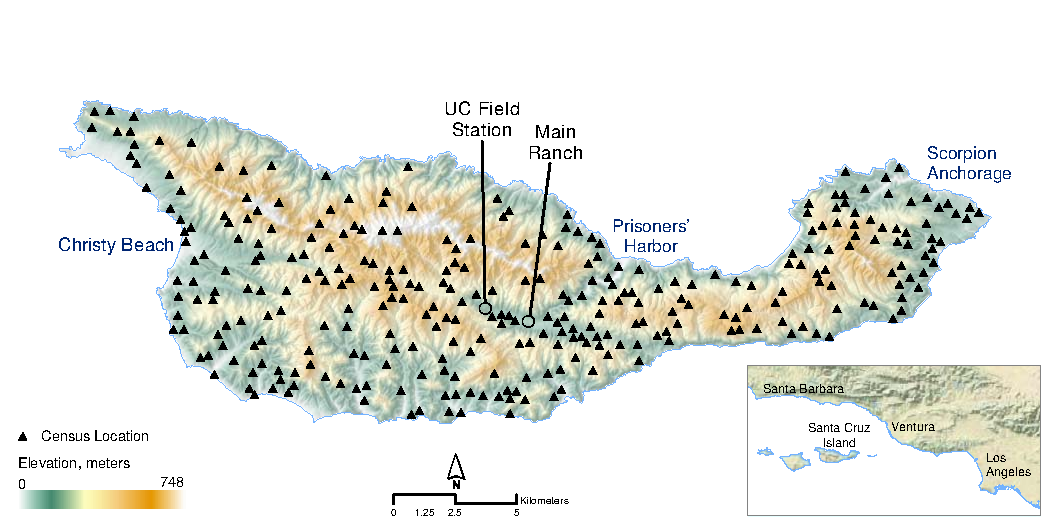
\includegraphics[width=0.8\textwidth]{figs/Santa-Cruz} \\
    Santa Cruz Island
  \end{center}
\end{frame}




\begin{frame}[fragile]
  \frametitle{Santa Cruz Data}
  \footnotesize


{\bf Habitat data for all 2787 grid cells covering the island}
\begin{knitrout}
\definecolor{shadecolor}{rgb}{0.878, 0.918, 0.933}\color{fgcolor}\begin{kframe}
\begin{alltt}
\hlkwd{head}\hlstd{(cruz2)}
\end{alltt}
\begin{verbatim}
##          x       y elevation forest chaparral habitat seeds
## 1 230736.7 3774324       241      0         0     Oak   Low
## 2 231036.7 3774324       323      0         0    Pine   Med
## 3 231336.7 3774324       277      0         0    Pine  High
## 4 230436.7 3774024        13      0         0     Oak   Med
## 5 230736.7 3774024       590      0         0     Oak  High
## 6 231036.7 3774024       533      0         0     Oak   Low
\end{verbatim}
\end{kframe}
\end{knitrout}
\end{frame}



\begin{frame}[fragile]
  \frametitle{Maps of predictor variables}
%  {\bf Elevation}
  \scriptsize

\includegraphics[width=\textwidth]{figure/elev-1}
\end{frame}




\begin{frame}[fragile]
  \frametitle{Maps of predictor variables}
%  {\bf Forest cover}
  \scriptsize

\includegraphics[width=\textwidth]{figure/forest-1}
\end{frame}






\begin{frame}
  \frametitle{Questions}
  \large
  \begin{enumerate}[<+- | visible@+->][\bf \color{PineGreen} (1)]
    \item How many jays are on the island?
    \item What environmental variables influence abundance?
    \item Can we predict consequences of environmental change?
  \end{enumerate}
\end{frame}



\begin{frame}[fragile]
  \frametitle{Maps of predictor variables}
%  {\bf Chaparral cover}

\includegraphics[width=\textwidth]{figure/plots-1}
\end{frame}




\begin{frame}[fragile]
  \frametitle{The (fake) jay data}
\begin{knitrout}\scriptsize
\definecolor{shadecolor}{rgb}{0.878, 0.918, 0.933}\color{fgcolor}\begin{kframe}
\begin{alltt}
\hlkwd{head}\hlstd{(jayData)}
\end{alltt}
\begin{verbatim}
##             x       y elevation forest chaparral habitat seeds jays
## 2345 258636.7 3764124       423   0.00      0.02     Oak   Med   34
## 740  261936.7 3769224       506   0.10      0.45     Oak   Med   38
## 2304 246336.7 3764124       859   0.00      0.26     Oak  High   40
## 2433 239436.7 3763524      1508   0.02      0.03    Pine   Med   43
## 1104 239436.7 3767724       483   0.26      0.37     Oak   Med   36
## 607  236436.7 3769524       830   0.00      0.01     Oak   Low   39
\end{verbatim}
\end{kframe}
\end{knitrout}
\end{frame}



\begin{frame}[fragile]
  \frametitle{Fit a model}
  \vspace{-2mm}
\begin{knitrout}\tiny
\definecolor{shadecolor}{rgb}{0.878, 0.918, 0.933}\color{fgcolor}\begin{kframe}
\begin{alltt}
\hlstd{fm6} \hlkwb{<-} \hlkwd{lm}\hlstd{(jays} \hlopt{~} \hlstd{habitat} \hlopt{*} \hlstd{seeds} \hlopt{+} \hlstd{elevation} \hlopt{+}
          \hlkwd{I}\hlstd{(elevation}\hlopt{^}\hlnum{2}\hlstd{)} \hlopt{+}  \hlstd{chaparral,} \hlkwc{data}\hlstd{=jayData)}
\hlkwd{summary}\hlstd{(fm6)}
\end{alltt}
\begin{verbatim}
## 
## Call:
## lm(formula = jays ~ habitat * seeds + elevation + I(elevation^2) + 
##     chaparral, data = jayData)
## 
## Residuals:
##     Min      1Q  Median      3Q     Max 
## -4.9796 -1.3642  0.0165  1.2872  4.0242 
## 
## Coefficients:
##                        Estimate Std. Error t value Pr(>|t|)    
## (Intercept)           2.796e+01  1.643e+00  17.018  < 2e-16 ***
## habitatOak            5.799e+00  1.640e+00   3.536 0.000651 ***
## habitatPine           3.858e+00  1.791e+00   2.155 0.033922 *  
## seedsLow              2.401e+00  2.081e+00   1.154 0.251667    
## seedsMed              1.784e+00  1.785e+00   0.999 0.320385    
## elevation             1.216e-02  2.240e-03   5.428 4.98e-07 ***
## I(elevation^2)       -2.551e-06  1.436e-06  -1.777 0.079105 .  
## chaparral             9.341e-01  1.053e+00   0.887 0.377579    
## habitatOak:seedsLow  -3.263e+00  2.276e+00  -1.434 0.155248    
## habitatPine:seedsLow -2.105e+00  2.450e+00  -0.859 0.392557    
## habitatOak:seedsMed  -3.384e+00  1.964e+00  -1.723 0.088337 .  
## habitatPine:seedsMed -2.749e+00  2.119e+00  -1.297 0.197860    
## ---
## Signif. codes:  0 '***' 0.001 '**' 0.01 '*' 0.05 '.' 0.1 ' ' 1
## 
## Residual standard error: 2.033 on 88 degrees of freedom
## Multiple R-squared:  0.7634,	Adjusted R-squared:  0.7338 
## F-statistic: 25.81 on 11 and 88 DF,  p-value: < 2.2e-16
\end{verbatim}
\end{kframe}
\end{knitrout}
\end{frame}



\begin{frame}[fragile]
  \frametitle{Predict jay abundance at each grid cell}
\begin{knitrout}
\definecolor{shadecolor}{rgb}{0.878, 0.918, 0.933}\color{fgcolor}\begin{kframe}
\begin{alltt}
\hlstd{E6} \hlkwb{<-} \hlkwd{predict}\hlstd{(fm6,} \hlkwc{type}\hlstd{=}\hlstr{"response"}\hlstd{,} \hlkwc{newdata}\hlstd{=cruz2,}
              \hlkwc{interval}\hlstd{=}\hlstr{"confidence"}\hlstd{)}
\end{alltt}
\end{kframe}
\end{knitrout}
\pause
\begin{knitrout}
\definecolor{shadecolor}{rgb}{0.878, 0.918, 0.933}\color{fgcolor}\begin{kframe}
\begin{alltt}
\hlstd{E6} \hlkwb{<-} \hlkwd{cbind}\hlstd{(cruz2[,}\hlkwd{c}\hlstd{(}\hlstr{"x"}\hlstd{,}\hlstr{"y"}\hlstd{)], E6)}
\hlkwd{head}\hlstd{(E6)}
\end{alltt}
\begin{verbatim}
##          x       y      fit      lwr      upr
## 1 230736.7 3774324 35.67687 34.34196 37.01177
## 2 231036.7 3774324 34.51169 33.45977 35.56361
## 3 231336.7 3774324 34.98846 32.93921 37.03770
## 4 230436.7 3774024 32.31463 30.76906 33.86021
## 5 230736.7 3774024 40.04266 38.27753 41.80780
## 6 231036.7 3774024 38.65059 37.41373 39.88745
\end{verbatim}
\end{kframe}
\end{knitrout}
\end{frame}


\begin{frame}[fragile]
  \frametitle{Map the predictions}
  \scriptsize

\includegraphics[width=\textwidth]{figure/Ejay-1}
\end{frame}




\begin{frame}[fragile]
  \frametitle{Map the predictions}
  \scriptsize

\includegraphics[width=\textwidth]{figure/Ljay-1}
\end{frame}




\begin{frame}[fragile]
  \frametitle{Map the predictions}
  \scriptsize

\includegraphics[width=\textwidth]{figure/Ujay-1}
\end{frame}




%% \begin{frame}[fragile]
%%   \frametitle{Future scenarios}
%%   {\bf What if the pine and oak disappear? \par}
%%   \pause
%%   \vspace{0.3cm}
%%   {\bf \dots assuming {\tt fm5} is the {\it correct} model}
%%   \pause
%%   \vspace{0.3cm}
%%   \footnotesize
%% <<>>=
%% future1 <- cruz2
%% future1$habitat[] <- "Bare"
%% future.pred1 <- predict(fm5, type="response", newdata=future1,
%%                         interval="confidence")
%% future.pred1 <- cbind(cruz2[,c("x","y")], future.pred1)
%% @
%% \end{frame}



\begin{frame}[fragile]
  \frametitle{Future scenarios}
  {\bf What if pine and oak disapper? \par}
  \scriptsize


\includegraphics[width=\textwidth]{figure/future1fig-1}
\end{frame}





%% \begin{frame}[fragile]
%%   \frametitle{Future scenarios}
%%   {\bf What if the island sinks 1000 m? \par}
%%   \vspace{0.3cm}
%% %  \pause
%% %  {\bf \dots assuming {\tt fm5} is the {\it correct} model}
%%   \pause
%%   \footnotesize
%% <<>>=
%% future2 <- cruz2
%% future2$elevation <- future2$elevation - 1000
%% future2$elevation[future2$elevation < 0] <- NA
%% future.pred2 <- predict(fm5, type="response", newdata=future2,
%%                         interval="confidence")
%% future.pred2 <- cbind(cruz2[,c("x","y")], future.pred2)
%% @
%% \end{frame}




\begin{frame}[fragile]
  \frametitle{Future scenarios}
  {\bf What if sea level rises? \par}
  \scriptsize
  \pause


\includegraphics[width=\textwidth]{figure/future2fig-1}
\end{frame}



%% \begin{frame}
%%   \frametitle{Worse yet \dots}
%%   \pause
%%   \huge
%%   What if our model is wrong?
%% \end{frame}



\end{document}

